\documentclass[11pt]{article}
\usepackage[utf8]{inputenc}
\usepackage[T1]{fontenc}
\usepackage{amsmath,amssymb}
\usepackage{graphicx}
\usepackage{booktabs}
\usepackage[margin=1in]{geometry}
\usepackage{microtype}
\setlength{\emergencystretch}{3em}
\usepackage[hidelinks]{hyperref}

\title{Phantom Mean Reversion: How Rolling Hedge Ratios Manufacture\\ Profits in Pairs-Trading Backtests}
\author{Rostyslav Shcherbyna\\ Independent researcher, Zaporizhzhia, Ukraine\\
\texttt{neozork@protonmail.com}\\
ORCID: \href{https://orcid.org/0009-0000-3773-5789}{0009-0000-3773-5789}}
\date{October 2026}

\begin{document}
\maketitle

\begin{abstract}
Pairs and statistical-arbitrage backtests often define the spread with a hedge ratio re-estimated on a rolling
window and book profit and loss (P\&L) as the position times the change of that spread. We show that this
accounting is not tradable: the change of a re-estimated spread contains a term generated by the re-estimation
itself, which no trader can earn. Because ordinary least squares refits the hedge so that recent residuals are
small, this term is systematically aligned with a z-score position and produces profits from nothing. On 400
pairs of independent Gaussian random walks---pairs with no relationship at all---a standard z-score rule booked
with spread-change accounting has a median annualized Sharpe ratio between $+4.4$ and $+14.8$ depending on the
window, positive on 100\% of the pairs, while the tradable P\&L of the same positions has a median Sharpe ratio
indistinguishable from zero. In a real cryptocurrency pairs strategy written with an AI coding assistant, the
artifact turned a reported Sharpe ratio of $+2.5$ to $+3.0$ into a tradable $-1.9$ to $-2.9$. The artifact passes
the usual statistical safeguards because it is a property of the accounting, not of the return series. It is not
specific to rolling least squares: it appears with exponentially weighted and Kalman-filter hedges, and it inflates the
Sharpe ratio even when the pair is genuinely cointegrated. We give the decomposition, a simulation that reproduces every
number, and two checks that detect it: re-deriving P\&L from leg positions, and running the strategy on independent
random walks. Both are implemented in the open-source Monte-Neo verifier.
\end{abstract}

\section{Introduction}

Pairs trading buys one asset and sells another in a ratio that makes the combination stationary, and trades
deviations of that combination from its mean \cite{vidyamurthy2004,gatev2006,krauss2017}. Since the relation between
assets drifts, practitioners commonly re-estimate the hedge ratio on a rolling window or with a Kalman filter
\cite{chan2013}. The spread is then $s_t = y_t - \beta_t x_t - \alpha_t$ with $(\alpha_t,\beta_t)$ fitted on data
up to time $t$, and a position is opened when the standardized spread is far from zero.

A short line of code makes such a backtest wrong: computing P\&L as
\begin{equation}
\text{PnL}_t^{\text{booked}} = q_{t-1}\,(s_t - s_{t-1}),
\label{eq:booked}
\end{equation}
where $q_{t-1}\in\{-1,0,1\}$ is the position in the spread decided at $t-1$. The formula looks natural---one
holds the spread, so one earns its change---but $s_t$ and $s_{t-1}$ are computed with different hedge ratios. The
portfolio actually held between $t-1$ and $t$ is $q_{t-1}$ units of $y$ and $-q_{t-1}\beta_{t-1}$ units of $x$. Its
P\&L is
\begin{equation}
\text{PnL}_t^{\text{tradable}} = q_{t-1}\,(\Delta y_t - \beta_{t-1}\,\Delta x_t).
\label{eq:tradable}
\end{equation}

We call the difference \emph{phantom mean reversion}. This paper makes four points: (i) the difference has a
simple closed form (Section~\ref{sec:decomp}); (ii) it is large and positive even when the two assets are
independent random walks (Section~\ref{sec:sim}); (iii) it passed the statistical gates of a real research pipeline (Section~\ref{sec:case}, an illustration); (iv) it is cheap to detect (Section~\ref{sec:detect}).

The phenomenon is related to, but distinct from, spurious regression between independent integrated series
\cite{granger1974,phillips1986}, which is also known to affect Kalman-filter state-space models \cite{eroglu2022}: there the fitted coefficient is meaningless; here, in addition, the refitting of
the coefficient leaks into the booked P\&L. It is also a different failure from look-ahead bias, since every
estimate uses only past and current data, and from backtest overfitting \cite{bailey2014pbo,bailey2014dsr},
since a single parameter setting suffices. Practitioner write-ups warn about hedge ratios estimated on the full sample
(which is look-ahead); the artifact studied here remains when every estimate is strictly causal. We are not aware of a
formal treatment of it.

\section{Decomposition}
\label{sec:decomp}

Write $\Delta\beta_t=\beta_t-\beta_{t-1}$ and $\Delta\alpha_t=\alpha_t-\alpha_{t-1}$. Then
\begin{equation}
s_t - s_{t-1} = (\Delta y_t - \beta_{t-1}\Delta x_t) - \Delta\beta_t\, x_t - \Delta\alpha_t,
\end{equation}
so that
\begin{equation}
\text{PnL}_t^{\text{booked}} - \text{PnL}_t^{\text{tradable}} = -\,q_{t-1}\,\bigl(\Delta\beta_t\, x_t + \Delta\alpha_t\bigr).
\label{eq:phantom}
\end{equation}
The right-hand side is the \emph{phantom term}. It involves no price change that a position could capture: it is
the effect of re-estimating $(\alpha,\beta)$ on the level of the spread.

Why is it positive on average? Let $\hat e_t=y_t-\beta_{t-1}x_t-\alpha_{t-1}$ be the residual of bar $t$ under the
hedge fitted one bar earlier, the residual a trader would have seen. Since $s_t-\hat e_t=-\Delta\beta_t x_t-\Delta\alpha_t$,
Eq.~\eqref{eq:phantom} can be written
\begin{equation}
\text{PnL}_t^{\text{booked}} - \text{PnL}_t^{\text{tradable}} = q_{t-1}\,(s_t-\hat e_t).
\end{equation}
The fit at $t$ contains the observation of bar $t$, so its residual is pulled toward zero relative to $\hat e_t$: for least
squares that adds one observation this is the leverage identity $s_t=(1-h_t)\,\hat e_t$, and a rolling window, which also
drops the oldest observation, behaves similarly. A z-score rule is short the spread when $s_{t-1}$ is high, i.e.\ when
$q_{t-1}=-1$, and $\hat e_t$ is then, because residuals are persistent, also high; so $s_t-\hat e_t<0$ and the term is
positive. The same holds with the signs reversed for a long position. In our simulations with $w=100$ the slope of $s_t$ on
$\hat e_t$ is $0.970$ and the correlation of $s_{t-1}$ with $\hat e_t$ is $0.970$ (\texttt{mechanism\_check.py}), so each bar
transfers about $3\%$ of the residual to the booked P\&L in the direction of the position, whether or not any price moved.
The shorter the window, the larger the leverage $h_t$ and the larger the artifact.

\section{Simulation on independent random walks}
\label{sec:sim}

\paragraph{Design.} For each of 400 pairs we draw two independent log-price random walks of 5000 bars with
Gaussian increments of standard deviation $0.01$. The hedge $(\alpha_t,\beta_t)$ is the OLS fit of $y$ on $x$
over the trailing window of $w$ bars ending at $t$ (inclusive; no look-ahead). The z-score is
$z_t=s_t/\hat\sigma_t$, with $\hat\sigma_t$ the in-window residual standard deviation. The position is $-1$ when
$z_t>2$, $+1$ when $z_t<-2$, and returns to $0$ when $|z_t|<0.5$. Sharpe ratios are annualized for hourly bars in
a market open all year ($\sqrt{8760}$). No costs are applied: the point is the sign, not the size, of the edge.
P\&L is measured in log-price units per unit of $y$. The seed and code are in the supplementary material; every number below is reproduced by \texttt{phantom\_mr\_sim.py}.

\begin{table}[htbp]
\centering
\begin{tabular}{rrrrrr}
\toprule
 & \multicolumn{2}{c}{Booked, Eq.~\eqref{eq:booked}} & \multicolumn{2}{c}{Tradable, Eq.~\eqref{eq:tradable}} & Phantom share\\
Window $w$ & median SR & positive & median SR & positive & of booked P\&L\\
\midrule
30  & $+14.81$ & 100\% & $-0.05$ & 48\% & 1.00\\
60  & $+11.53$ & 100\% & $-0.07$ & 48\% & 1.00\\
100 & $+9.27$  & 100\% & $-0.01$ & 50\% & 1.00\\
250 & $+5.98$  & 100\% & $-0.01$ & 50\% & 1.02\\
500 & $+4.39$  & 100\% & $+0.13$ & 55\% & 0.98\\
\bottomrule
\end{tabular}
\caption{Annualized Sharpe ratios over 400 pairs of independent random walks (seed 20261015). The 5th
percentile of the booked Sharpe ratio is $+13.37$, $+10.26$, $+7.86$, $+4.63$ and $+3.06$ for the five windows.
``Positive'' is the share of pairs with a positive Sharpe ratio. ``Phantom share'' is the sum of the phantom term divided by the sum of booked P\&L over all pairs.}
\label{tab:sim}
\end{table}

\paragraph{Results.} Table~\ref{tab:sim} and Figure~\ref{fig:window} show that the booked P\&L is profitable on
every pair for every window, with the artifact decreasing as the window grows. The tradable P\&L of exactly the
same positions has a median Sharpe ratio between $-0.07$ and $+0.13$ and is positive on about half of the pairs,
as it must be for independent assets (the standard error of a median Sharpe ratio over 400 paths is roughly $0.1$, so $+0.13$ is within sampling error). Essentially all booked profit is phantom. Figure~\ref{fig:path} shows a
single pair: the booked equity curve rises smoothly while the tradable curve wanders around zero.

\begin{figure}[htbp]
\centering
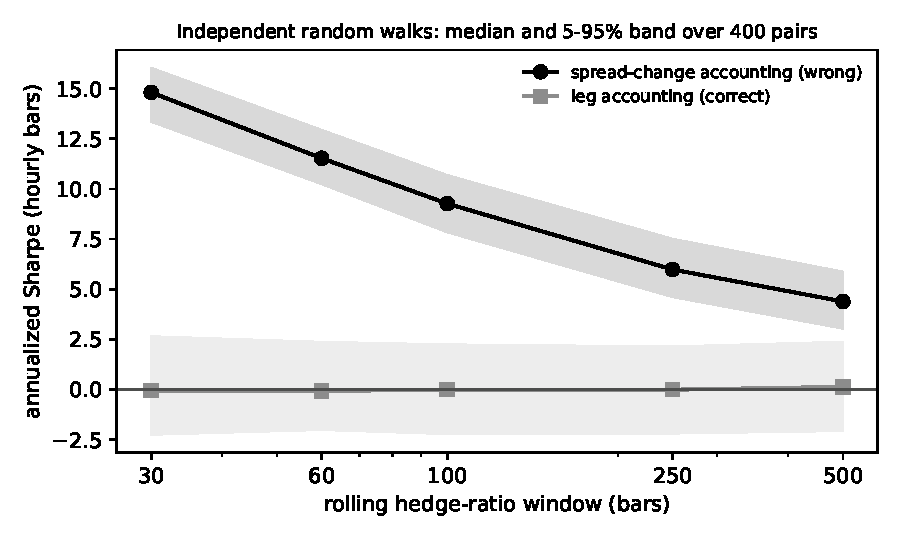
\includegraphics[width=0.8\linewidth]{figures/fig1_sharpe_vs_window.pdf}
\caption{Median annualized Sharpe ratio and 5--95\% band versus the rolling window.}
\label{fig:window}
\end{figure}

\begin{figure}[htbp]
\centering
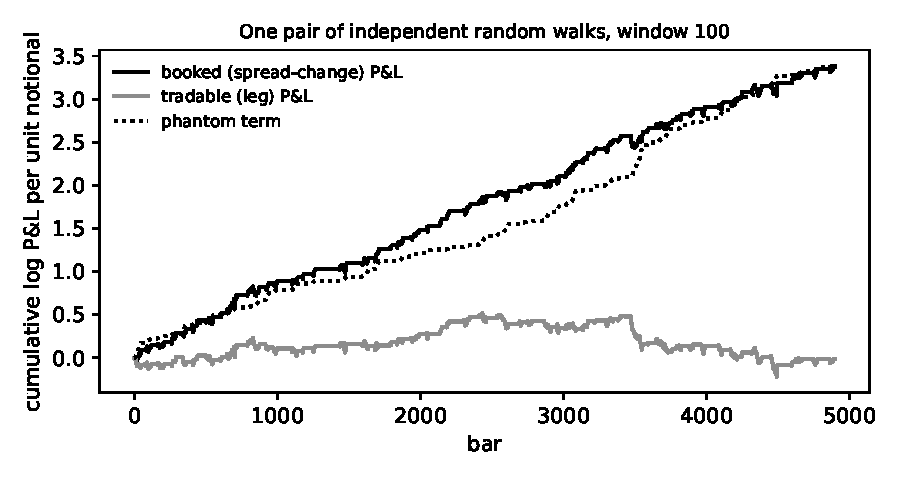
\includegraphics[width=0.8\linewidth]{figures/fig2_example_path.pdf}
\caption{Cumulative booked, tradable and phantom P\&L for one pair of independent random walks ($w=100$).}
\label{fig:path}
\end{figure}

\section{Other hedge estimators and real mean reversion}
\label{sec:robust}

Two objections arise. First, the artifact might be specific to rolling least squares. Second, it might vanish when the
pair really mean-reverts. Table~\ref{tab:other} addresses both with the same design as Section~\ref{sec:sim} (400 pairs of
5000 bars, seed 20261015, a 250-bar warm-up for all rows, no costs; \texttt{other\_hedges.py}). Exponentially weighted
least squares (weights decaying by one half every 50 or 250 bars) and a Kalman filter with a random-walk state for $(\alpha,\beta)$ \cite{elliott2005} (state noise $\delta/(1-\delta)$, observation variance $10^{-4}$) behave like the rolling fit: on independent walks the booked Sharpe ratio is positive on every pair and the tradable one on about half of them. With the Kalman filter the effect needs a slowly moving hedge ($\delta=10^{-5}$); for larger
$\delta$ the filter tracks every deviation and in our runs the z-score (the forecast error scaled by its predicted standard deviation) never reaches the entry threshold, so no pair trades and there is nothing to book. The last two rows use a genuinely cointegrated pair, $y_t=x_t+e_t$ with $e_t$ an AR(1) process
($\varphi=0.95$). The rule is then truly profitable (tradable Sharpe $+7.6$ and $+8.8$), but the booked Sharpe ratio is
still larger, and $41\%$ and $11\%$ of the booked profit is phantom. The artifact therefore does not require the absence of
a real edge: it inflates a real one.

\begin{table}[htbp]
\centering
\begin{tabular}{lrrr}
\toprule
Hedge estimator, pair & booked SR & tradable SR & phantom share\\
\midrule
rolling OLS, $w=100$, independent walks & $+9.25$ & $-0.03$ & 1.00\\
EWMA OLS, half-life 50, independent & $+6.17$ & $-0.08$ & 1.01\\
EWMA OLS, half-life 250, independent & $+3.29$ & $+0.05$ & 1.00\\
Kalman, $\delta=10^{-5}$, independent & $+12.67$ & $+0.13$ & 1.00\\
Kalman, $\delta=10^{-4}$ or $10^{-3}$, independent & \multicolumn{3}{c}{no pair trades}\\
rolling OLS, $w=100$, cointegrated & $+12.80$ & $+7.57$ & 0.41\\
rolling OLS, $w=500$, cointegrated & $+9.84$ & $+8.79$ & 0.11\\
\bottomrule
\end{tabular}
\caption{Median annualized Sharpe ratios (SR) over 400 pairs. Booked is positive on 100\% of the pairs in every row;
tradable is positive on 48--54\% of the independent pairs and on 100\% of the cointegrated ones.}
\label{tab:other}
\end{table}

\section{Case study: a cryptocurrency pairs strategy}
\label{sec:case}

The artifact was found in the author's own research. A z-score reversion strategy on hourly prices of
alternative cryptocurrencies against Bitcoin, with a rolling hedge ratio and intercept, was written with an AI
coding assistant and reviewed by the author. With spread-change accounting, it reported annualized Sharpe ratios
of $+3.01$, $+2.92$ and $+2.56$ under funding costs of zero, one and five times the observed rate, and it passed the
pipeline's statistical gates. A backtest verifier given only the return series (the author's own tool, Monte-Neo, before the checks of
Section~\ref{sec:detect} existed) rated it ``usable with warnings''.
Recomputing P\&L from the legs, Eq.~\eqref{eq:tradable}, gave $-1.95$, $-2.15$ and $-2.94$; the gross Sharpe
ratio at zero cost was $-0.94$, the out-of-sample Sharpe ratio $-3.07$, and the same rule on a second exchange
gave $-1.40$. The strategy was rejected. The strategy and its data are private, so this case is an illustration, not
evidence: the evidence is the simulation of Sections~\ref{sec:sim} and~\ref{sec:robust}, which anyone can rerun.

The episode illustrates why the artifact is dangerous: statistical tests on the return series---deflated Sharpe
ratio, multiple-testing corrections, bootstrap confidence intervals---assume that the series is what a trader
would have earned. Phantom mean reversion violates that assumption before any statistics are computed. The
smoothness of the booked equity curve, which usually reassures, is itself a symptom.

\section{Detection}
\label{sec:detect}

\paragraph{Re-derive P\&L from leg positions.} Store the quantity held in each leg and recompute P\&L as the sum
over legs of quantity times price change. Any strategy whose reported P\&L differs from this re-derivation by more
than costs has an accounting error. For a spread strategy booked from spread changes the difference is exactly the phantom term,
Eq.~\eqref{eq:phantom}, and its share of total P\&L is an informative diagnostic.

\paragraph{Random-walk null test.} Run the unchanged strategy code on pairs of independent random walks matched
in length and volatility. A correct implementation must earn a Sharpe ratio indistinguishable from zero there.
A strategy that is reliably profitable on independent random walks has a defect in its accounting or its data
handling, regardless of what it does on real data. This test needs no knowledge of the defect and also catches
other mechanical edges.

\paragraph{Implementation.} Both checks are implemented in the open-source verifier Monte-Neo (MIT licence, version
0.54.0), developed by the author:
\begin{itemize}
\item \texttt{monte-neo verify -{}-legs legs.csv} re-derives the P\&L from a table of prices and quantities held in each
leg and fails the check \texttt{accounting\_mismatch} when more than 5\% of the reported P\&L is unexplained;
\item \texttt{monte-neo verify -{}-null-test pairs.py:pnl} runs a strategy on independent random walks and fails
\texttt{edge\_on\_noise} when more than 75\% of the paths are profitable and the median $t$-statistic of the mean return
exceeds one.
\end{itemize}
On the single simulated pair of the repository example ($w=100$, 4899 bars) the first check reports a Sharpe ratio of
$+8.58$ against $-0.44$ for the legs (the unexplained share is $105\%$ because the legs lose money) and writes the
corrected return series; the second, with hourly annualization, gives a median Sharpe ratio of $+9.04$ (100\% of 100 paths
positive) for the wrong booking and $-0.22$ ($44\%$ positive) for the correct one. The commands and files are in the
directory \texttt{examples/phantom\_pairs} of the repository.

\paragraph{Two simpler checks.} Freezing the hedge ratio for the life of each trade removes the artifact; so does
computing the spread for bar $t$ with $(\alpha_{t-1},\beta_{t-1})$ when evaluating P\&L. A large gap between the
two versions of a backtest is a warning.

\section{Discussion}

The artifact needs only three ingredients---a re-estimated hedge, a position in the spread, and P\&L booked from
spread changes---and Section~\ref{sec:robust} shows it for rolling OLS, exponentially weighted regressions and a
slowly moving Kalman-filter hedge, all of which move $(\alpha_t,\beta_t)$ toward recent observations. Strategies that
fix the hedge at entry, or that book P\&L from the legs, are not affected. As backtests are
increasingly written by AI coding assistants and checked by statistical tests on their outputs, accounting
errors of this kind deserve explicit tests: they produce exactly the smooth, significant results that such
pipelines are built to reward. We recommend that backtest verifiers accept leg positions, not only returns, and
include the random-walk null test as a standard trap.

\paragraph{Limitations.} The simulations use Gaussian random walks, one z-score rule with fixed thresholds, hourly
annualization and no costs: they show the sign and the order of magnitude of the artifact, not its size in a given
market. Costs would reduce the booked profit, but it exists before any cost is charged and no trader can earn it. The detection checks find an accounting
error in the reported P\&L; they do not show that a strategy has an edge.

\paragraph{Reproducibility.} \texttt{phantom\_mr\_sim.py} (numpy only) reproduces Table~\ref{tab:sim},
\texttt{other\_hedges.py} reproduces Table~\ref{tab:other}, \texttt{mechanism\_check.py} the two numbers of Section~\ref{sec:decomp} and \texttt{make\_figures.py} the figures. The code, the results files and this manuscript are in the repository
\url{https://github.com/NeoZorK/Monte-Neo}, release \texttt{v0.54.0}, under
\url{paper/phantom-mean-reversion}.

\paragraph{Competing interests.} The author develops Monte-Neo, mentioned in Section~\ref{sec:detect}. The work had no
funding.

\begin{thebibliography}{12}
\bibitem{bailey2014pbo} D.~H. Bailey, J.~M. Borwein, M.~L\'opez de Prado and Q.~J. Zhu. The probability of
backtest overfitting. \emph{Journal of Computational Finance}, 20(4):39--69, 2017.
\bibitem{bailey2014dsr} D.~H. Bailey and M.~L\'opez de Prado. The deflated Sharpe ratio: correcting for
selection bias, backtest overfitting and non-normality. \emph{Journal of Portfolio Management}, 40(5):94--107, 2014.
\bibitem{chan2013} E.~P. Chan. \emph{Algorithmic Trading: Winning Strategies and Their Rationale}. Wiley, 2013.
\bibitem{elliott2005} R.~J. Elliott, J.~van der Hoek and W.~P. Malcolm. Pairs trading. \emph{Quantitative Finance}, 5(3):271--276, 2005.
\bibitem{eroglu2022} B.~A. Ero\u{g}lu, J.~I. Miller and T.~M. Y\i\u{g}it. Time-varying cointegration and the Kalman
filter. \emph{Econometric Reviews}, 41(1):1--21, 2022.
\bibitem{gatev2006} E.~Gatev, W.~N. Goetzmann and K.~G. Rouwenhorst. Pairs trading: performance of a
relative-value arbitrage rule. \emph{Review of Financial Studies}, 19(3):797--827, 2006.
\bibitem{granger1974} C.~W.~J. Granger and P.~Newbold. Spurious regressions in econometrics. \emph{Journal of
Econometrics}, 2(2):111--120, 1974.
\bibitem{krauss2017} C.~Krauss. Statistical arbitrage pairs trading strategies: review and outlook. \emph{Journal of
Economic Surveys}, 31(2):513--545, 2017.
\bibitem{phillips1986} P.~C.~B. Phillips. Understanding spurious regressions in econometrics. \emph{Journal of
Econometrics}, 33(3):311--340, 1986.
\bibitem{vidyamurthy2004} G.~Vidyamurthy. \emph{Pairs Trading: Quantitative Methods and Analysis}. Wiley, 2004.
\end{thebibliography}

\end{document}
